\documentclass[a4paper,landscape,english,12pt]{article}
\usepackage{../Common/AstroReport}
\begin{document}
\AstroCover{Workflow}{1.0}

\section*{About this document}
This document contains a detailed and illustrated guideline on how to get astrophotography done at our own style
\section{Workflow}
\begin{multicols}{2}
	
\subsection{Setting the mount on station}
\begin{enumerate}
	\item In advance, prepare your observation plan, choose a target, study its movement along the sky and decide the timing for imaging. An application such as  \myhttp{Stellarium}{https://stellarium-web.org/} could be helpful to previsualize the sky and the movement of the target (Figure \ref{fig:stellarium})
	
	%\begin{figure}[hbt]
	%\includegraphics[width=10cm]{../Figures/ecliptic.jpg}
	%\caption{Using the app Stellarium to prepare the observation}		
	%\label{fig:stellarium}
	%\end{figure} 
	
	\item Choose a convenient observation spot and make sure you accurately identify the orientation of North, South, West, and East. Also, check that here is a good observability of the target, lack of visual obstacles and visibility of Polaris Star (at the north, Figures \ref{fig:polaris1} and \ref{fig:polaris2})). A smartphone with a "Compass" app might be very handy (Figure \ref{fig:compass}).+
	
	\item Level the tripod such that the equatorial base is perfectly horizontal in both axis: N-S, W-E In this case too, a "Level" app (Figure \ref{fig:level}) could help to find the perfect horizontal.
	
	\item Check the weight balance of the mount and the main gear. Find the balance in both AR and DEC rotation axis. In the case of RA, leave a slight bias to the west in the AR axis so that its rotation would be easier.
	
	\item Complete the polar alignment procedure
	\begin{enumerate}
		\item Us an app such as "Polar finder" to know he position of Polaris within reticule of the mount
		\item Using the knobs designed for this, move the mount such as Polaris appears right in the position described in the app.
		\end{enumerate}
	\item Now the mount is on station. Remember these three important steps, finding a good level of the tripod, balancing the weight and polar alignment, as a strong requirement to succeed in the imaging stage.
\end{enumerate}

\newpage\subsection{Calibrating everything}

For a good imaging session, all the steps must be given with the maximum accuracy. Starting from the cameras which are to be used. 

\subsubsection{Calibrating the main camera }

It is very important for the main camera to be perfectly focused and not only to the naked eye, it must be further. In order to do that

\subsubsection{Calibrating the guide camera }

\subsubsection{Calibrating the smartphone for assisted "goto"}

\subsubsection{Calibrating the guiding software}


\subsection{Imaging}


\subsection{Postprocessing}

\section{The software}

\subsection{Stellarium}

\subsection{EKOS}

\subsection{PHD2}

\subsection{ASTAP}

\subsection{Astrometry.net}

\subsection{Siril}

\subsection{GIMP}

\subsection{GraXpert}

\begin{enumerate}
	\item 
\end{enumerate}


\end{multicols}

%\newpage\newpage\pagecolor{black}\color{white}
\ \\\section{Andromeda Galaxy}
\includegraphics[width=\textwidth]{/home/lcv/Dropbox/AstroPhotography/Imaging/Original/Andromeda_Galaxy.jpg}
{\footnotesize\color{white}
The Andromeda Galaxy is a barred spiral galaxy and is the nearest major galaxy to the Milky Way. It was originally named the Andromeda Nebula and is cataloged as Messier 31, M31, and NGC 224. Andromeda has a D25 isophotal diameter of about 46.56 kiloparsecs (152,000 light-years)[8] and is approximately 765 kpc (2.5 million light-years) from Earth. The galaxy's name stems from the area of Earth's sky in which it appears, the constellation of Andromeda, which itself is named after the princess who was the wife of Perseus in Greek mythology. 


}\ \\
\includegraphics[width=\textwidth]{/home/lcv/Dropbox/AstroPhotography/Imaging/Grayscale/Andromeda_Galaxy.jpg}
\begin{center}
 \ \newpage
\includegraphics[width=0.75\textwidth]{/home/lcv/Dropbox/AstroPhotography/Imaging/Annotated/Andromeda_Galaxy_Annotated.jpg}

\includegraphics[height=4cm]{/home/lcv/Dropbox/AstroPhotography/Imaging/Annotated/Andromeda_Galaxy_Hist}
\includegraphics[height=4cm]{/home/lcv/Dropbox/AstroPhotography/Imaging/Annotated/Andromeda_Galaxy_Globe.jpg}
\includegraphics[height=4cm]{/home/lcv/Dropbox/AstroPhotography/Imaging/Annotated/Andromeda_Galaxy_Close.jpg}
\includegraphics[height=4cm]{/home/lcv/Dropbox/AstroPhotography/Imaging/Annotated/Andromeda_Galaxy_Closer.jpg}
\end{center}
\ \\\section{Bubble Nebula}
\includegraphics[width=\textwidth]{/home/lcv/Dropbox/AstroPhotography/Imaging/Original/Bubble_Nebula.jpg}
{\footnotesize\color{white}
NGC 7635, also known as the Bubble Nebula, Sharpless 162, or Caldwell 11, is an H II region emission nebula in the constellation Cassiopeia. It lies close to the open cluster Messier 52. The "bubble" is created by the stellar wind from a massive hot, 8.7 magnitude young central star, SAO 20575 (BD+60°2522). The nebula is near a giant molecular cloud which contains the expansion of the bubble nebula while itself being excited by the hot central star, causing it to glow. It was discovered in November 1787 by William Herschel. The star BD+60°2522 is thought to have a mass of about 44 M


}\ \\
\includegraphics[width=\textwidth]{/home/lcv/Dropbox/AstroPhotography/Imaging/Grayscale/Bubble_Nebula.jpg}
\begin{center}
 \ \newpage
\includegraphics[width=0.75\textwidth]{/home/lcv/Dropbox/AstroPhotography/Imaging/Annotated/Bubble_Nebula_Annotated.jpg}

\includegraphics[height=4cm]{/home/lcv/Dropbox/AstroPhotography/Imaging/Annotated/Bubble_Nebula_Hist}
\includegraphics[height=4cm]{/home/lcv/Dropbox/AstroPhotography/Imaging/Annotated/Bubble_Nebula_Globe.jpg}
\includegraphics[height=4cm]{/home/lcv/Dropbox/AstroPhotography/Imaging/Annotated/Bubble_Nebula_Close.jpg}
\includegraphics[height=4cm]{/home/lcv/Dropbox/AstroPhotography/Imaging/Annotated/Bubble_Nebula_Closer.jpg}
\end{center}
\ \\\section{California Nebula}
\includegraphics[width=\textwidth]{/home/lcv/Dropbox/AstroPhotography/Imaging/Original/California_Nebula.jpg}
{\footnotesize\color{white}
The California Nebula (Also known NGC 1499 or Sh2-220) is an emission nebula located in the constellation Perseus. Its name comes from its resemblance to the outline of the US State of California in long exposure photographs. It is almost 2.5° long on the sky and, because of its very low surface brightness, it is extremely difficult to observe visually. It can be observed with a Hα filter (isolates the Hα line at 656 nm) or Hβ filter (isolates the Hβ line at 486 nm) in a rich-field telescope under dark skies.[2] It lies at a distance of about 1,000 light years from Earth. Its fluorescence is due to excitation of the Hβ line in the nebula by the nearby prodigiously energetic O7 star, Xi Persei (also known as Menkib).[3]


}\ \\
\includegraphics[width=\textwidth]{/home/lcv/Dropbox/AstroPhotography/Imaging/Grayscale/California_Nebula.jpg}
\begin{center}
 \ \newpage
\includegraphics[width=0.75\textwidth]{/home/lcv/Dropbox/AstroPhotography/Imaging/Annotated/California_Nebula_Annotated.jpg}

\includegraphics[height=4cm]{/home/lcv/Dropbox/AstroPhotography/Imaging/Annotated/California_Nebula_Hist}
\includegraphics[height=4cm]{/home/lcv/Dropbox/AstroPhotography/Imaging/Annotated/California_Nebula_Globe.jpg}
\includegraphics[height=4cm]{/home/lcv/Dropbox/AstroPhotography/Imaging/Annotated/California_Nebula_Close.jpg}
\includegraphics[height=4cm]{/home/lcv/Dropbox/AstroPhotography/Imaging/Annotated/California_Nebula_Closer.jpg}
\end{center}
\ \\\section{Dumbbell Nebula}
\includegraphics[width=\textwidth]{/home/lcv/Dropbox/AstroPhotography/Imaging/Original/Dumbbell_Nebula.jpg}
{\footnotesize\color{white}


}\ \\
\includegraphics[width=\textwidth]{/home/lcv/Dropbox/AstroPhotography/Imaging/Grayscale/Dumbbell_Nebula.jpg}
\begin{center}
 \ \newpage
\includegraphics[width=0.75\textwidth]{/home/lcv/Dropbox/AstroPhotography/Imaging/Annotated/Dumbbell_Nebula_Annotated.jpg}

\includegraphics[height=4cm]{/home/lcv/Dropbox/AstroPhotography/Imaging/Annotated/Dumbbell_Nebula_Hist}
\includegraphics[height=4cm]{/home/lcv/Dropbox/AstroPhotography/Imaging/Annotated/Dumbbell_Nebula_Globe.jpg}
\includegraphics[height=4cm]{/home/lcv/Dropbox/AstroPhotography/Imaging/Annotated/Dumbbell_Nebula_Close.jpg}
\includegraphics[height=4cm]{/home/lcv/Dropbox/AstroPhotography/Imaging/Annotated/Dumbbell_Nebula_Closer.jpg}
\end{center}
\ \\\section{Eagle Nebula}
\includegraphics[width=\textwidth]{/home/lcv/Dropbox/AstroPhotography/Imaging/Original/Eagle_Nebula.jpg}
{\footnotesize\color{white}


}\ \\
\includegraphics[width=\textwidth]{/home/lcv/Dropbox/AstroPhotography/Imaging/Grayscale/Eagle_Nebula.jpg}
\begin{center}
 \ \newpage
\includegraphics[width=0.75\textwidth]{/home/lcv/Dropbox/AstroPhotography/Imaging/Annotated/Eagle_Nebula_Annotated.jpg}

\includegraphics[height=4cm]{/home/lcv/Dropbox/AstroPhotography/Imaging/Annotated/Eagle_Nebula_Hist}
\includegraphics[height=4cm]{/home/lcv/Dropbox/AstroPhotography/Imaging/Annotated/Eagle_Nebula_Globe.jpg}
\includegraphics[height=4cm]{/home/lcv/Dropbox/AstroPhotography/Imaging/Annotated/Eagle_Nebula_Close.jpg}
\includegraphics[height=4cm]{/home/lcv/Dropbox/AstroPhotography/Imaging/Annotated/Eagle_Nebula_Closer.jpg}
\end{center}
\ \\\section{Eastern Veil Nebula}
\includegraphics[width=\textwidth]{/home/lcv/Dropbox/AstroPhotography/Imaging/Original/Eastern_Veil_Nebula.jpg}
{\footnotesize\color{white}


}\ \\
\includegraphics[width=\textwidth]{/home/lcv/Dropbox/AstroPhotography/Imaging/Grayscale/Eastern_Veil_Nebula.jpg}
\begin{center}
 \ \newpage
\includegraphics[width=0.75\textwidth]{/home/lcv/Dropbox/AstroPhotography/Imaging/Annotated/Eastern_Veil_Nebula_Annotated.jpg}

\includegraphics[height=4cm]{/home/lcv/Dropbox/AstroPhotography/Imaging/Annotated/Eastern_Veil_Nebula_Globe.jpg}
\includegraphics[height=4cm]{/home/lcv/Dropbox/AstroPhotography/Imaging/Annotated/Eastern_Veil_Nebula_Close.jpg}
\includegraphics[height=4cm]{/home/lcv/Dropbox/AstroPhotography/Imaging/Annotated/Eastern_Veil_Nebula_Closer.jpg}
\end{center}
\ \\\section{Fireworks Galaxy}
\includegraphics[width=\textwidth]{/home/lcv/Dropbox/AstroPhotography/Imaging/Original/Fireworks_Galaxy.jpg}
{\footnotesize\color{white}


}\ \\
\includegraphics[width=\textwidth]{/home/lcv/Dropbox/AstroPhotography/Imaging/Grayscale/Fireworks_Galaxy.jpg}
\begin{center}
 \ \newpage
\includegraphics[width=0.75\textwidth]{/home/lcv/Dropbox/AstroPhotography/Imaging/Annotated/Fireworks_Galaxy_Annotated.jpg}

\includegraphics[height=4cm]{/home/lcv/Dropbox/AstroPhotography/Imaging/Annotated/Fireworks_Galaxy_Globe.jpg}
\includegraphics[height=4cm]{/home/lcv/Dropbox/AstroPhotography/Imaging/Annotated/Fireworks_Galaxy_Close.jpg}
\includegraphics[height=4cm]{/home/lcv/Dropbox/AstroPhotography/Imaging/Annotated/Fireworks_Galaxy_Closer.jpg}
\end{center}
\ \\\section{Full Veil Nebula}
\includegraphics[width=\textwidth]{/home/lcv/Dropbox/AstroPhotography/Imaging/Original/Full_Veil_Nebula.jpg}
{\footnotesize\color{white}


}\ \\
\begin{center}
 \ \newpage
\includegraphics[width=0.75\textwidth]{/home/lcv/Dropbox/AstroPhotography/Imaging/Annotated/Full_Veil_Nebula_Annotated.jpg}

\includegraphics[height=4cm]{/home/lcv/Dropbox/AstroPhotography/Imaging/Annotated/Full_Veil_Nebula_Globe.jpg}
\includegraphics[height=4cm]{/home/lcv/Dropbox/AstroPhotography/Imaging/Annotated/Full_Veil_Nebula_Close.jpg}
\end{center}
\ \\\section{Ghost Of Cassiopeia}
\includegraphics[width=\textwidth]{/home/lcv/Dropbox/AstroPhotography/Imaging/Original/Ghost_Of_Cassiopeia.jpg}
{\footnotesize\color{white}


}\ \\
\includegraphics[width=\textwidth]{/home/lcv/Dropbox/AstroPhotography/Imaging/Grayscale/Ghost_Of_Cassiopeia.jpg}
\begin{center}
 \ \newpage
\includegraphics[width=0.75\textwidth]{/home/lcv/Dropbox/AstroPhotography/Imaging/Annotated/Ghost_Of_Cassiopeia_Annotated.jpg}

\includegraphics[height=4cm]{/home/lcv/Dropbox/AstroPhotography/Imaging/Annotated/Ghost_Of_Cassiopeia_Globe.jpg}
\includegraphics[height=4cm]{/home/lcv/Dropbox/AstroPhotography/Imaging/Annotated/Ghost_Of_Cassiopeia_Close.jpg}
\includegraphics[height=4cm]{/home/lcv/Dropbox/AstroPhotography/Imaging/Annotated/Ghost_Of_Cassiopeia_Closer.jpg}
\end{center}
\ \\\section{HD225526}
\includegraphics[width=\textwidth]{/home/lcv/Dropbox/AstroPhotography/Imaging/Original/HD225526.jpg}
{\footnotesize\color{white}


}\ \\
\includegraphics[width=\textwidth]{/home/lcv/Dropbox/AstroPhotography/Imaging/Grayscale/HD225526.jpg}
\begin{center}
 \ \newpage
\includegraphics[width=0.75\textwidth]{/home/lcv/Dropbox/AstroPhotography/Imaging/Annotated/HD225526_Annotated.jpg}

\includegraphics[height=4cm]{/home/lcv/Dropbox/AstroPhotography/Imaging/Annotated/HD225526_Globe.jpg}
\includegraphics[height=4cm]{/home/lcv/Dropbox/AstroPhotography/Imaging/Annotated/HD225526_Close.jpg}
\includegraphics[height=4cm]{/home/lcv/Dropbox/AstroPhotography/Imaging/Annotated/HD225526_Closer.jpg}
\end{center}
\ \\\section{Heart Nebula}
\includegraphics[width=\textwidth]{/home/lcv/Dropbox/AstroPhotography/Imaging/Original/Heart_Nebula.jpg}
{\footnotesize\color{white}


}\ \\
\includegraphics[width=\textwidth]{/home/lcv/Dropbox/AstroPhotography/Imaging/Grayscale/Heart_Nebula.jpg}
\begin{center}
 \ \newpage
\includegraphics[width=0.75\textwidth]{/home/lcv/Dropbox/AstroPhotography/Imaging/Annotated/Heart_Nebula_Annotated.jpg}

\includegraphics[height=4cm]{/home/lcv/Dropbox/AstroPhotography/Imaging/Annotated/Heart_Nebula_Globe.jpg}
\includegraphics[height=4cm]{/home/lcv/Dropbox/AstroPhotography/Imaging/Annotated/Heart_Nebula_Close.jpg}
\includegraphics[height=4cm]{/home/lcv/Dropbox/AstroPhotography/Imaging/Annotated/Heart_Nebula_Closer.jpg}
\end{center}
\ \\\section{Helix Nebula}
\includegraphics[width=\textwidth]{/home/lcv/Dropbox/AstroPhotography/Imaging/Original/Helix_Nebula.jpg}
{\footnotesize\color{white}


}\ \\
\includegraphics[width=\textwidth]{/home/lcv/Dropbox/AstroPhotography/Imaging/Grayscale/Helix_Nebula.jpg}
\begin{center}
 \ \newpage
\includegraphics[width=0.75\textwidth]{/home/lcv/Dropbox/AstroPhotography/Imaging/Annotated/Helix_Nebula_Annotated.jpg}

\includegraphics[height=4cm]{/home/lcv/Dropbox/AstroPhotography/Imaging/Annotated/Helix_Nebula_Globe.jpg}
\includegraphics[height=4cm]{/home/lcv/Dropbox/AstroPhotography/Imaging/Annotated/Helix_Nebula_Close.jpg}
\includegraphics[height=4cm]{/home/lcv/Dropbox/AstroPhotography/Imaging/Annotated/Helix_Nebula_Closer.jpg}
\end{center}
\ \\\section{Horse Head Nebula}
\includegraphics[width=\textwidth]{/home/lcv/Dropbox/AstroPhotography/Imaging/Original/Horse_Head_Nebula.jpg}
{\footnotesize\color{white}


}\ \\
\includegraphics[width=\textwidth]{/home/lcv/Dropbox/AstroPhotography/Imaging/Grayscale/Horse_Head_Nebula.jpg}
\begin{center}
 \ \newpage
\includegraphics[width=0.75\textwidth]{/home/lcv/Dropbox/AstroPhotography/Imaging/Annotated/Horse_Head_Nebula_Annotated.jpg}

\includegraphics[height=4cm]{/home/lcv/Dropbox/AstroPhotography/Imaging/Annotated/Horse_Head_Nebula_Globe.jpg}
\includegraphics[height=4cm]{/home/lcv/Dropbox/AstroPhotography/Imaging/Annotated/Horse_Head_Nebula_Close.jpg}
\includegraphics[height=4cm]{/home/lcv/Dropbox/AstroPhotography/Imaging/Annotated/Horse_Head_Nebula_Closer.jpg}
\end{center}
\ \\\section{Iris Nebula}
\includegraphics[width=\textwidth]{/home/lcv/Dropbox/AstroPhotography/Imaging/Original/Iris_Nebula.jpg}
{\footnotesize\color{white}


}\ \\
\includegraphics[width=\textwidth]{/home/lcv/Dropbox/AstroPhotography/Imaging/Grayscale/Iris_Nebula.jpg}
\begin{center}
 \ \newpage
\includegraphics[width=0.75\textwidth]{/home/lcv/Dropbox/AstroPhotography/Imaging/Annotated/Iris_Nebula_Annotated.jpg}

\includegraphics[height=4cm]{/home/lcv/Dropbox/AstroPhotography/Imaging/Annotated/Iris_Nebula_Globe.jpg}
\includegraphics[height=4cm]{/home/lcv/Dropbox/AstroPhotography/Imaging/Annotated/Iris_Nebula_Close.jpg}
\includegraphics[height=4cm]{/home/lcv/Dropbox/AstroPhotography/Imaging/Annotated/Iris_Nebula_Closer.jpg}
\end{center}
\ \\\section{Lagoon Nebula}
\includegraphics[width=\textwidth]{/home/lcv/Dropbox/AstroPhotography/Imaging/Original/Lagoon_Nebula.jpg}
{\footnotesize\color{white}


}\ \\
\includegraphics[width=\textwidth]{/home/lcv/Dropbox/AstroPhotography/Imaging/Grayscale/Lagoon_Nebula.jpg}
\begin{center}
 \ \newpage
\includegraphics[width=0.75\textwidth]{/home/lcv/Dropbox/AstroPhotography/Imaging/Annotated/Lagoon_Nebula_Annotated.jpg}

\includegraphics[height=4cm]{/home/lcv/Dropbox/AstroPhotography/Imaging/Annotated/Lagoon_Nebula_Globe.jpg}
\includegraphics[height=4cm]{/home/lcv/Dropbox/AstroPhotography/Imaging/Annotated/Lagoon_Nebula_Close.jpg}
\includegraphics[height=4cm]{/home/lcv/Dropbox/AstroPhotography/Imaging/Annotated/Lagoon_Nebula_Closer.jpg}
\end{center}
\ \\\section{Pacman Nebula}
\includegraphics[width=\textwidth]{/home/lcv/Dropbox/AstroPhotography/Imaging/Original/Pacman_Nebula.jpg}
{\footnotesize\color{white}


}\ \\
\includegraphics[width=\textwidth]{/home/lcv/Dropbox/AstroPhotography/Imaging/Grayscale/Pacman_Nebula.jpg}
\begin{center}
 \ \newpage
\includegraphics[width=0.75\textwidth]{/home/lcv/Dropbox/AstroPhotography/Imaging/Annotated/Pacman_Nebula_Annotated.jpg}

\includegraphics[height=4cm]{/home/lcv/Dropbox/AstroPhotography/Imaging/Annotated/Pacman_Nebula_Globe.jpg}
\includegraphics[height=4cm]{/home/lcv/Dropbox/AstroPhotography/Imaging/Annotated/Pacman_Nebula_Close.jpg}
\includegraphics[height=4cm]{/home/lcv/Dropbox/AstroPhotography/Imaging/Annotated/Pacman_Nebula_Closer.jpg}
\end{center}
\ \\\section{Pleiades Cluster}
\includegraphics[width=\textwidth]{/home/lcv/Dropbox/AstroPhotography/Imaging/Original/Pleiades_Cluster.jpg}
{\footnotesize\color{white}


}\ \\
\includegraphics[width=\textwidth]{/home/lcv/Dropbox/AstroPhotography/Imaging/Grayscale/Pleiades_Cluster.jpg}
\begin{center}
 \ \newpage
\includegraphics[width=0.75\textwidth]{/home/lcv/Dropbox/AstroPhotography/Imaging/Annotated/Pleiades_Cluster_Annotated.jpg}

\includegraphics[height=4cm]{/home/lcv/Dropbox/AstroPhotography/Imaging/Annotated/Pleiades_Cluster_Globe.jpg}
\includegraphics[height=4cm]{/home/lcv/Dropbox/AstroPhotography/Imaging/Annotated/Pleiades_Cluster_Close.jpg}
\includegraphics[height=4cm]{/home/lcv/Dropbox/AstroPhotography/Imaging/Annotated/Pleiades_Cluster_Closer.jpg}
\end{center}
\ \\\section{Swann Nebula}
\includegraphics[width=\textwidth]{/home/lcv/Dropbox/AstroPhotography/Imaging/Original/Swann_Nebula.jpg}
{\footnotesize\color{white}


}\ \\
\includegraphics[width=\textwidth]{/home/lcv/Dropbox/AstroPhotography/Imaging/Grayscale/Swann_Nebula.jpg}
\begin{center}
 \ \newpage
\includegraphics[width=0.75\textwidth]{/home/lcv/Dropbox/AstroPhotography/Imaging/Annotated/Swann_Nebula_Annotated.jpg}

\includegraphics[height=4cm]{/home/lcv/Dropbox/AstroPhotography/Imaging/Annotated/Swann_Nebula_Globe.jpg}
\includegraphics[height=4cm]{/home/lcv/Dropbox/AstroPhotography/Imaging/Annotated/Swann_Nebula_Close.jpg}
\includegraphics[height=4cm]{/home/lcv/Dropbox/AstroPhotography/Imaging/Annotated/Swann_Nebula_Closer.jpg}
\end{center}
\ \\\section{The Moon}
\includegraphics[width=\textwidth]{/home/lcv/Dropbox/AstroPhotography/Imaging/Original/The_Moon.jpg}
{\footnotesize\color{white}


}\ \\
\begin{center}
\end{center}
\ \\\section{Triangulum Galaxy}
\includegraphics[width=\textwidth]{/home/lcv/Dropbox/AstroPhotography/Imaging/Original/Triangulum_Galaxy.jpg}
{\footnotesize\color{white}


}\ \\
\includegraphics[width=\textwidth]{/home/lcv/Dropbox/AstroPhotography/Imaging/Grayscale/Triangulum_Galaxy.jpg}
\begin{center}
 \ \newpage
\includegraphics[width=0.75\textwidth]{/home/lcv/Dropbox/AstroPhotography/Imaging/Annotated/Triangulum_Galaxy_Annotated.jpg}

\includegraphics[height=4cm]{/home/lcv/Dropbox/AstroPhotography/Imaging/Annotated/Triangulum_Galaxy_Globe.jpg}
\includegraphics[height=4cm]{/home/lcv/Dropbox/AstroPhotography/Imaging/Annotated/Triangulum_Galaxy_Close.jpg}
\includegraphics[height=4cm]{/home/lcv/Dropbox/AstroPhotography/Imaging/Annotated/Triangulum_Galaxy_Closer.jpg}
\end{center}
\ \\\section{Trifid Nebula}
\includegraphics[width=\textwidth]{/home/lcv/Dropbox/AstroPhotography/Imaging/Original/Trifid_Nebula.jpg}
{\footnotesize\color{white}


}\ \\
\includegraphics[width=\textwidth]{/home/lcv/Dropbox/AstroPhotography/Imaging/Grayscale/Trifid_Nebula.jpg}
\begin{center}
 \ \newpage
\includegraphics[width=0.75\textwidth]{/home/lcv/Dropbox/AstroPhotography/Imaging/Annotated/Trifid_Nebula_Annotated.jpg}

\includegraphics[height=4cm]{/home/lcv/Dropbox/AstroPhotography/Imaging/Annotated/Trifid_Nebula_Globe.jpg}
\includegraphics[height=4cm]{/home/lcv/Dropbox/AstroPhotography/Imaging/Annotated/Trifid_Nebula_Close.jpg}
\includegraphics[height=4cm]{/home/lcv/Dropbox/AstroPhotography/Imaging/Annotated/Trifid_Nebula_Closer.jpg}
\end{center}
\ \\\section{Vega Star}
\includegraphics[width=\textwidth]{/home/lcv/Dropbox/AstroPhotography/Imaging/Original/Vega_Star.jpg}
{\footnotesize\color{white}


}\ \\
\includegraphics[width=\textwidth]{/home/lcv/Dropbox/AstroPhotography/Imaging/Grayscale/Vega_Star.jpg}
\begin{center}
 \ \newpage
\includegraphics[width=0.75\textwidth]{/home/lcv/Dropbox/AstroPhotography/Imaging/Annotated/Vega_Star_Annotated.jpg}

\includegraphics[height=4cm]{/home/lcv/Dropbox/AstroPhotography/Imaging/Annotated/Vega_Star_Globe.jpg}
\includegraphics[height=4cm]{/home/lcv/Dropbox/AstroPhotography/Imaging/Annotated/Vega_Star_Close.jpg}
\includegraphics[height=4cm]{/home/lcv/Dropbox/AstroPhotography/Imaging/Annotated/Vega_Star_Closer.jpg}
\end{center}
\ \\\section{Western Veil Nebula}
\includegraphics[width=\textwidth]{/home/lcv/Dropbox/AstroPhotography/Imaging/Original/Western_Veil_Nebula.jpg}
{\footnotesize\color{white}


}\ \\
\includegraphics[width=\textwidth]{/home/lcv/Dropbox/AstroPhotography/Imaging/Grayscale/Western_Veil_Nebula.jpg}
\begin{center}
 \ \newpage
\includegraphics[width=0.75\textwidth]{/home/lcv/Dropbox/AstroPhotography/Imaging/Annotated/Western_Veil_Nebula_Annotated.jpg}

\includegraphics[height=4cm]{/home/lcv/Dropbox/AstroPhotography/Imaging/Annotated/Western_Veil_Nebula_Globe.jpg}
\includegraphics[height=4cm]{/home/lcv/Dropbox/AstroPhotography/Imaging/Annotated/Western_Veil_Nebula_Close.jpg}
\includegraphics[height=4cm]{/home/lcv/Dropbox/AstroPhotography/Imaging/Annotated/Western_Veil_Nebula_Closer.jpg}
\end{center}
\ \\\section{Wizard Nebula}
\includegraphics[width=\textwidth]{/home/lcv/Dropbox/AstroPhotography/Imaging/Original/Wizard_Nebula.jpg}
{\footnotesize\color{white}


}\ \\
\includegraphics[width=\textwidth]{/home/lcv/Dropbox/AstroPhotography/Imaging/Grayscale/Wizard_Nebula.jpg}
\begin{center}
 \ \newpage
\includegraphics[width=0.75\textwidth]{/home/lcv/Dropbox/AstroPhotography/Imaging/Annotated/Wizard_Nebula_Annotated.jpg}

\includegraphics[height=4cm]{/home/lcv/Dropbox/AstroPhotography/Imaging/Annotated/Wizard_Nebula_Close.jpg}
\includegraphics[height=4cm]{/home/lcv/Dropbox/AstroPhotography/Imaging/Annotated/Wizard_Nebula_Closer.jpg}
\end{center}


\newpage

\section{Figures}
	\begin{figure}[hbt]
	\includegraphics[width=5cm]{../Figures/ecliptic.jpg}
	\caption{Using the app Stellarium to prepare the observation}		
	\label{fig:stellarium}
\end{figure} 

\begin{figure}[hbt]
	\includegraphics[width=5cm]{../Figures/compass.jpg}
	\includegraphics[width=5cm]{../Figures/compass.jpg}
	\caption{Using the app "Compass" to prepare the observation}		
	\label{fig:compass}
\end{figure} 

\begin{figure}[hbt]
	\includegraphics[width=5cm]{../Figures/level.jpg}
	\caption{Using the app "Level" to prepare the observation}		
	\label{fig:level}
\end{figure} 

\begin{figure}[hbt]
	\includegraphics[width=5cm]{../Figures/polarallignment.jpg}
	\caption{Using the app "Level" to prepare the observation}		
	\label{fig:polaralign}
\end{figure} 

\begin{figure}[hbt]
	\includegraphics[width=5cm]{../Figures/Polaris-1.jpg}
	\caption{One way to find Polaris. This method depends on your geographical position}		
	\label{fig:polaris1}
\end{figure} 


\begin{figure}[hbt]
	\includegraphics[width=5cm]{../Figures/Polaris-2.jpg}
	\caption{A second way to find Polaris which does not depend on your geographical position}		
	\label{fig:polaris2}
\end{figure} 


\end{document}


CALIBRADO
Calibrar cámara primaria
Modo Manual
AWB en tugnsten
Herramienta de enfocado de EKOS para enfoque fino
Hacer fotos a 1-5 segundos y máxima exposición 
Hasta que el factor SNR esté por debajo de 2 (por lo menos) en todas las estrellas clasificadas
Calibrar cámara de guiado
Si es webcam, comprobar que están conectadas e identificadas
v4l2-ctl --list-devices
Comprobar en EKOS que el puerto de la cámara es correcto
Si es necesario resetear los parámetros, usar guvcview para restablecer de fabrica
guvcview -d /dev/videoX
Si no está enfocada, enfocar a un objeto muy brillante y enfocar de forma gruesa. Luego usar EKOS para enfoque fino.
Ajustar la luz.En general
Poner alpha al máximo
Poner sharpness al mínimo
Poner a 0 la compensación de retroiluminación
Poner saturación al nivel medio
Poner Hue/Color al nivel medio
Ir subiendo la luz y el contraste hasta encontrar el máximo de estrellas
Ajustar el apilado simulado
Si son exposiciones de menos de 1 seg entonces usar apilado aditivo, si no, apilado por la media porque es el que da un SNR más estable para el autoguiado, sobre todo por las condiciones locales del seeing
Ajustar la resolución de captura al máximo
Poner exposición automática, incluso forzarla desde la línea de comandos
v4l2-ctl -d /dev/video4 -c auto_exposure=3
v4l2-ctl -d /dev/video4 -c auto_exposure=3 --try-fmt-video colorspace=srgb
Calibrar smartphone goto
Con la cámara,
Apuntar a un objeto muy brillante y conocido
Colocarlo lo más en el centro posible
Con el smartphone
Bloquear giro de la pantalla
Calibrar la brújula del smartphone
Colocar smartphone en su peana
Arrancar stellarium y centrar en el mismo objeto anterior, con esto tendremos la máxima precisión a la que podemos aspirar en el posicionamiento cerca del objetivo
Calibrar autoguiado  PHD2
Seleccionar un objeto ligeramente por encima de la eclíptica
Conectar la cámara de guiado y la montura a PHD2
Muestrear imágenes y ver que se encuentran bien las estrellas. Cuantas más mejor. 
Si es necesario, recalibrar la cámara de guiado
Calibrar PHD2
CENTRAR EL OBJETIVO
Aproximación inicial
Buscar el objetivo en stellarium del smartphone
Liberar frenos de RA y DEC y colocar el objetivo en el centro de la pantalla del smartphone
Volver a colocar los frenos
Aproximación final visual
Buscar el objetivo en Stellarium-web y colocar  al FPV 2.9 para reconocer el campo
Tomar muestra a 2-3 s y buscar referencias para ir centrando
Cuidado de evitar manchas de polvo en el sensor
Aproximación final asistida con Astrometría web
Tomar muestra a 5-10 segundos
Subirla a Astrometry.net y esperar plate solving
Tomar referencias, ajustar el centrado y repetir hasta que el objetivo esté centrado
Aproximación final asistida con Astrometría local ASTAP
Abrir ASTAP y cargar la imagen que queremos calibrar
Poner stretch a 8/HIGH
SOLVE
Mostrar capas de Deep Space Objects y retícula A/H
MUESTREO
Comprobar centrado en FITS
Arrancar autoguiado
Muestrear en NATIVE con exposiciones cada vez más largas, 10 s, 30s, 60 s, 90 s, 120 s
Si el autoguiado está bien, programar número de capturas y comenzar la captura
PREPROCESADO 
Siempre: comprobar histograma con forma de Gauss,
Ojo saturación blanco y/o negro a izquierda y derecha del histograma
Descargar la secuencia con todas las capturas
Siril
Debayer
Preprocesado: los dark y flats: optimize
Registrado
Elegir una foto de la secuencia que sea la referencia: bien enfocada y con el objetivo centrado.
Global Star+ bilineal
Apilado: recompute+[Average staking with rejection+Additive with scaling+roundess | nstars]+Sigma Clipping+Ouput Norm + RGB Eq
Eliminar ruido verde
Si es posible Calibración Fotométrica del Color
Enmarcar y crop
Stretch, auto o manual
Salvar base em disco
Graxpert
Primer denoise sin saturación
saturacion 1.5-1.8
Grabar sin stretch
Siril
Eliminar fondo (si es necesario)
Starnet y eliminar estrellas
Graxpert (starless)
denoise sin saturación
saturacion 1.5
Grabar sin stretch
Gimp (starless)
Si mucho ruido de fondo
Ajustar ruido de fondo con EXPOSURE para nivelar ruido. Bajar nivel de negro
Colors - Levels: oscurecer
SI es necesario, Highlights: bajar nivel
SI mucho ruido aún) Graxpert (starless), denoise sin saturar
Saturar el color para dar más contraste
- Perfilar
- Denoise
- Si mucho ruido: gradiente
- Realzar con stretch CURVAS o contraste
- Ajustar highlight

- Gimp (starmask)
- 
\newpage

\newpage\pagecolor{black}\color{white}
\ \\\section{Andromeda Galaxy}
\includegraphics[width=\textwidth]{/home/lcv/Dropbox/AstroPhotography/Imaging/Original/Andromeda_Galaxy.jpg}
{\footnotesize\color{white}
The Andromeda Galaxy is a barred spiral galaxy and is the nearest major galaxy to the Milky Way. It was originally named the Andromeda Nebula and is cataloged as Messier 31, M31, and NGC 224. Andromeda has a D25 isophotal diameter of about 46.56 kiloparsecs (152,000 light-years)[8] and is approximately 765 kpc (2.5 million light-years) from Earth. The galaxy's name stems from the area of Earth's sky in which it appears, the constellation of Andromeda, which itself is named after the princess who was the wife of Perseus in Greek mythology. 


}\ \\
\includegraphics[width=\textwidth]{/home/lcv/Dropbox/AstroPhotography/Imaging/Grayscale/Andromeda_Galaxy.jpg}
\begin{center}
 \ \newpage
\includegraphics[width=0.75\textwidth]{/home/lcv/Dropbox/AstroPhotography/Imaging/Annotated/Andromeda_Galaxy_Annotated.jpg}

\includegraphics[height=4cm]{/home/lcv/Dropbox/AstroPhotography/Imaging/Annotated/Andromeda_Galaxy_Hist}
\includegraphics[height=4cm]{/home/lcv/Dropbox/AstroPhotography/Imaging/Annotated/Andromeda_Galaxy_Globe.jpg}
\includegraphics[height=4cm]{/home/lcv/Dropbox/AstroPhotography/Imaging/Annotated/Andromeda_Galaxy_Close.jpg}
\includegraphics[height=4cm]{/home/lcv/Dropbox/AstroPhotography/Imaging/Annotated/Andromeda_Galaxy_Closer.jpg}
\end{center}
\ \\\section{Bubble Nebula}
\includegraphics[width=\textwidth]{/home/lcv/Dropbox/AstroPhotography/Imaging/Original/Bubble_Nebula.jpg}
{\footnotesize\color{white}
NGC 7635, also known as the Bubble Nebula, Sharpless 162, or Caldwell 11, is an H II region emission nebula in the constellation Cassiopeia. It lies close to the open cluster Messier 52. The "bubble" is created by the stellar wind from a massive hot, 8.7 magnitude young central star, SAO 20575 (BD+60°2522). The nebula is near a giant molecular cloud which contains the expansion of the bubble nebula while itself being excited by the hot central star, causing it to glow. It was discovered in November 1787 by William Herschel. The star BD+60°2522 is thought to have a mass of about 44 M


}\ \\
\includegraphics[width=\textwidth]{/home/lcv/Dropbox/AstroPhotography/Imaging/Grayscale/Bubble_Nebula.jpg}
\begin{center}
 \ \newpage
\includegraphics[width=0.75\textwidth]{/home/lcv/Dropbox/AstroPhotography/Imaging/Annotated/Bubble_Nebula_Annotated.jpg}

\includegraphics[height=4cm]{/home/lcv/Dropbox/AstroPhotography/Imaging/Annotated/Bubble_Nebula_Hist}
\includegraphics[height=4cm]{/home/lcv/Dropbox/AstroPhotography/Imaging/Annotated/Bubble_Nebula_Globe.jpg}
\includegraphics[height=4cm]{/home/lcv/Dropbox/AstroPhotography/Imaging/Annotated/Bubble_Nebula_Close.jpg}
\includegraphics[height=4cm]{/home/lcv/Dropbox/AstroPhotography/Imaging/Annotated/Bubble_Nebula_Closer.jpg}
\end{center}
\ \\\section{California Nebula}
\includegraphics[width=\textwidth]{/home/lcv/Dropbox/AstroPhotography/Imaging/Original/California_Nebula.jpg}
{\footnotesize\color{white}
The California Nebula (Also known NGC 1499 or Sh2-220) is an emission nebula located in the constellation Perseus. Its name comes from its resemblance to the outline of the US State of California in long exposure photographs. It is almost 2.5° long on the sky and, because of its very low surface brightness, it is extremely difficult to observe visually. It can be observed with a Hα filter (isolates the Hα line at 656 nm) or Hβ filter (isolates the Hβ line at 486 nm) in a rich-field telescope under dark skies.[2] It lies at a distance of about 1,000 light years from Earth. Its fluorescence is due to excitation of the Hβ line in the nebula by the nearby prodigiously energetic O7 star, Xi Persei (also known as Menkib).[3]


}\ \\
\includegraphics[width=\textwidth]{/home/lcv/Dropbox/AstroPhotography/Imaging/Grayscale/California_Nebula.jpg}
\begin{center}
 \ \newpage
\includegraphics[width=0.75\textwidth]{/home/lcv/Dropbox/AstroPhotography/Imaging/Annotated/California_Nebula_Annotated.jpg}

\includegraphics[height=4cm]{/home/lcv/Dropbox/AstroPhotography/Imaging/Annotated/California_Nebula_Hist}
\includegraphics[height=4cm]{/home/lcv/Dropbox/AstroPhotography/Imaging/Annotated/California_Nebula_Globe.jpg}
\includegraphics[height=4cm]{/home/lcv/Dropbox/AstroPhotography/Imaging/Annotated/California_Nebula_Close.jpg}
\includegraphics[height=4cm]{/home/lcv/Dropbox/AstroPhotography/Imaging/Annotated/California_Nebula_Closer.jpg}
\end{center}
\ \\\section{Dumbbell Nebula}
\includegraphics[width=\textwidth]{/home/lcv/Dropbox/AstroPhotography/Imaging/Original/Dumbbell_Nebula.jpg}
{\footnotesize\color{white}


}\ \\
\includegraphics[width=\textwidth]{/home/lcv/Dropbox/AstroPhotography/Imaging/Grayscale/Dumbbell_Nebula.jpg}
\begin{center}
 \ \newpage
\includegraphics[width=0.75\textwidth]{/home/lcv/Dropbox/AstroPhotography/Imaging/Annotated/Dumbbell_Nebula_Annotated.jpg}

\includegraphics[height=4cm]{/home/lcv/Dropbox/AstroPhotography/Imaging/Annotated/Dumbbell_Nebula_Hist}
\includegraphics[height=4cm]{/home/lcv/Dropbox/AstroPhotography/Imaging/Annotated/Dumbbell_Nebula_Globe.jpg}
\includegraphics[height=4cm]{/home/lcv/Dropbox/AstroPhotography/Imaging/Annotated/Dumbbell_Nebula_Close.jpg}
\includegraphics[height=4cm]{/home/lcv/Dropbox/AstroPhotography/Imaging/Annotated/Dumbbell_Nebula_Closer.jpg}
\end{center}
\ \\\section{Eagle Nebula}
\includegraphics[width=\textwidth]{/home/lcv/Dropbox/AstroPhotography/Imaging/Original/Eagle_Nebula.jpg}
{\footnotesize\color{white}


}\ \\
\includegraphics[width=\textwidth]{/home/lcv/Dropbox/AstroPhotography/Imaging/Grayscale/Eagle_Nebula.jpg}
\begin{center}
 \ \newpage
\includegraphics[width=0.75\textwidth]{/home/lcv/Dropbox/AstroPhotography/Imaging/Annotated/Eagle_Nebula_Annotated.jpg}

\includegraphics[height=4cm]{/home/lcv/Dropbox/AstroPhotography/Imaging/Annotated/Eagle_Nebula_Hist}
\includegraphics[height=4cm]{/home/lcv/Dropbox/AstroPhotography/Imaging/Annotated/Eagle_Nebula_Globe.jpg}
\includegraphics[height=4cm]{/home/lcv/Dropbox/AstroPhotography/Imaging/Annotated/Eagle_Nebula_Close.jpg}
\includegraphics[height=4cm]{/home/lcv/Dropbox/AstroPhotography/Imaging/Annotated/Eagle_Nebula_Closer.jpg}
\end{center}
\ \\\section{Eastern Veil Nebula}
\includegraphics[width=\textwidth]{/home/lcv/Dropbox/AstroPhotography/Imaging/Original/Eastern_Veil_Nebula.jpg}
{\footnotesize\color{white}


}\ \\
\includegraphics[width=\textwidth]{/home/lcv/Dropbox/AstroPhotography/Imaging/Grayscale/Eastern_Veil_Nebula.jpg}
\begin{center}
 \ \newpage
\includegraphics[width=0.75\textwidth]{/home/lcv/Dropbox/AstroPhotography/Imaging/Annotated/Eastern_Veil_Nebula_Annotated.jpg}

\includegraphics[height=4cm]{/home/lcv/Dropbox/AstroPhotography/Imaging/Annotated/Eastern_Veil_Nebula_Globe.jpg}
\includegraphics[height=4cm]{/home/lcv/Dropbox/AstroPhotography/Imaging/Annotated/Eastern_Veil_Nebula_Close.jpg}
\includegraphics[height=4cm]{/home/lcv/Dropbox/AstroPhotography/Imaging/Annotated/Eastern_Veil_Nebula_Closer.jpg}
\end{center}
\ \\\section{Fireworks Galaxy}
\includegraphics[width=\textwidth]{/home/lcv/Dropbox/AstroPhotography/Imaging/Original/Fireworks_Galaxy.jpg}
{\footnotesize\color{white}


}\ \\
\includegraphics[width=\textwidth]{/home/lcv/Dropbox/AstroPhotography/Imaging/Grayscale/Fireworks_Galaxy.jpg}
\begin{center}
 \ \newpage
\includegraphics[width=0.75\textwidth]{/home/lcv/Dropbox/AstroPhotography/Imaging/Annotated/Fireworks_Galaxy_Annotated.jpg}

\includegraphics[height=4cm]{/home/lcv/Dropbox/AstroPhotography/Imaging/Annotated/Fireworks_Galaxy_Globe.jpg}
\includegraphics[height=4cm]{/home/lcv/Dropbox/AstroPhotography/Imaging/Annotated/Fireworks_Galaxy_Close.jpg}
\includegraphics[height=4cm]{/home/lcv/Dropbox/AstroPhotography/Imaging/Annotated/Fireworks_Galaxy_Closer.jpg}
\end{center}
\ \\\section{Full Veil Nebula}
\includegraphics[width=\textwidth]{/home/lcv/Dropbox/AstroPhotography/Imaging/Original/Full_Veil_Nebula.jpg}
{\footnotesize\color{white}


}\ \\
\begin{center}
 \ \newpage
\includegraphics[width=0.75\textwidth]{/home/lcv/Dropbox/AstroPhotography/Imaging/Annotated/Full_Veil_Nebula_Annotated.jpg}

\includegraphics[height=4cm]{/home/lcv/Dropbox/AstroPhotography/Imaging/Annotated/Full_Veil_Nebula_Globe.jpg}
\includegraphics[height=4cm]{/home/lcv/Dropbox/AstroPhotography/Imaging/Annotated/Full_Veil_Nebula_Close.jpg}
\end{center}
\ \\\section{Ghost Of Cassiopeia}
\includegraphics[width=\textwidth]{/home/lcv/Dropbox/AstroPhotography/Imaging/Original/Ghost_Of_Cassiopeia.jpg}
{\footnotesize\color{white}


}\ \\
\includegraphics[width=\textwidth]{/home/lcv/Dropbox/AstroPhotography/Imaging/Grayscale/Ghost_Of_Cassiopeia.jpg}
\begin{center}
 \ \newpage
\includegraphics[width=0.75\textwidth]{/home/lcv/Dropbox/AstroPhotography/Imaging/Annotated/Ghost_Of_Cassiopeia_Annotated.jpg}

\includegraphics[height=4cm]{/home/lcv/Dropbox/AstroPhotography/Imaging/Annotated/Ghost_Of_Cassiopeia_Globe.jpg}
\includegraphics[height=4cm]{/home/lcv/Dropbox/AstroPhotography/Imaging/Annotated/Ghost_Of_Cassiopeia_Close.jpg}
\includegraphics[height=4cm]{/home/lcv/Dropbox/AstroPhotography/Imaging/Annotated/Ghost_Of_Cassiopeia_Closer.jpg}
\end{center}
\ \\\section{HD225526}
\includegraphics[width=\textwidth]{/home/lcv/Dropbox/AstroPhotography/Imaging/Original/HD225526.jpg}
{\footnotesize\color{white}


}\ \\
\includegraphics[width=\textwidth]{/home/lcv/Dropbox/AstroPhotography/Imaging/Grayscale/HD225526.jpg}
\begin{center}
 \ \newpage
\includegraphics[width=0.75\textwidth]{/home/lcv/Dropbox/AstroPhotography/Imaging/Annotated/HD225526_Annotated.jpg}

\includegraphics[height=4cm]{/home/lcv/Dropbox/AstroPhotography/Imaging/Annotated/HD225526_Globe.jpg}
\includegraphics[height=4cm]{/home/lcv/Dropbox/AstroPhotography/Imaging/Annotated/HD225526_Close.jpg}
\includegraphics[height=4cm]{/home/lcv/Dropbox/AstroPhotography/Imaging/Annotated/HD225526_Closer.jpg}
\end{center}
\ \\\section{Heart Nebula}
\includegraphics[width=\textwidth]{/home/lcv/Dropbox/AstroPhotography/Imaging/Original/Heart_Nebula.jpg}
{\footnotesize\color{white}


}\ \\
\includegraphics[width=\textwidth]{/home/lcv/Dropbox/AstroPhotography/Imaging/Grayscale/Heart_Nebula.jpg}
\begin{center}
 \ \newpage
\includegraphics[width=0.75\textwidth]{/home/lcv/Dropbox/AstroPhotography/Imaging/Annotated/Heart_Nebula_Annotated.jpg}

\includegraphics[height=4cm]{/home/lcv/Dropbox/AstroPhotography/Imaging/Annotated/Heart_Nebula_Globe.jpg}
\includegraphics[height=4cm]{/home/lcv/Dropbox/AstroPhotography/Imaging/Annotated/Heart_Nebula_Close.jpg}
\includegraphics[height=4cm]{/home/lcv/Dropbox/AstroPhotography/Imaging/Annotated/Heart_Nebula_Closer.jpg}
\end{center}
\ \\\section{Helix Nebula}
\includegraphics[width=\textwidth]{/home/lcv/Dropbox/AstroPhotography/Imaging/Original/Helix_Nebula.jpg}
{\footnotesize\color{white}


}\ \\
\includegraphics[width=\textwidth]{/home/lcv/Dropbox/AstroPhotography/Imaging/Grayscale/Helix_Nebula.jpg}
\begin{center}
 \ \newpage
\includegraphics[width=0.75\textwidth]{/home/lcv/Dropbox/AstroPhotography/Imaging/Annotated/Helix_Nebula_Annotated.jpg}

\includegraphics[height=4cm]{/home/lcv/Dropbox/AstroPhotography/Imaging/Annotated/Helix_Nebula_Globe.jpg}
\includegraphics[height=4cm]{/home/lcv/Dropbox/AstroPhotography/Imaging/Annotated/Helix_Nebula_Close.jpg}
\includegraphics[height=4cm]{/home/lcv/Dropbox/AstroPhotography/Imaging/Annotated/Helix_Nebula_Closer.jpg}
\end{center}
\ \\\section{Horse Head Nebula}
\includegraphics[width=\textwidth]{/home/lcv/Dropbox/AstroPhotography/Imaging/Original/Horse_Head_Nebula.jpg}
{\footnotesize\color{white}


}\ \\
\includegraphics[width=\textwidth]{/home/lcv/Dropbox/AstroPhotography/Imaging/Grayscale/Horse_Head_Nebula.jpg}
\begin{center}
 \ \newpage
\includegraphics[width=0.75\textwidth]{/home/lcv/Dropbox/AstroPhotography/Imaging/Annotated/Horse_Head_Nebula_Annotated.jpg}

\includegraphics[height=4cm]{/home/lcv/Dropbox/AstroPhotography/Imaging/Annotated/Horse_Head_Nebula_Globe.jpg}
\includegraphics[height=4cm]{/home/lcv/Dropbox/AstroPhotography/Imaging/Annotated/Horse_Head_Nebula_Close.jpg}
\includegraphics[height=4cm]{/home/lcv/Dropbox/AstroPhotography/Imaging/Annotated/Horse_Head_Nebula_Closer.jpg}
\end{center}
\ \\\section{Iris Nebula}
\includegraphics[width=\textwidth]{/home/lcv/Dropbox/AstroPhotography/Imaging/Original/Iris_Nebula.jpg}
{\footnotesize\color{white}


}\ \\
\includegraphics[width=\textwidth]{/home/lcv/Dropbox/AstroPhotography/Imaging/Grayscale/Iris_Nebula.jpg}
\begin{center}
 \ \newpage
\includegraphics[width=0.75\textwidth]{/home/lcv/Dropbox/AstroPhotography/Imaging/Annotated/Iris_Nebula_Annotated.jpg}

\includegraphics[height=4cm]{/home/lcv/Dropbox/AstroPhotography/Imaging/Annotated/Iris_Nebula_Globe.jpg}
\includegraphics[height=4cm]{/home/lcv/Dropbox/AstroPhotography/Imaging/Annotated/Iris_Nebula_Close.jpg}
\includegraphics[height=4cm]{/home/lcv/Dropbox/AstroPhotography/Imaging/Annotated/Iris_Nebula_Closer.jpg}
\end{center}
\ \\\section{Lagoon Nebula}
\includegraphics[width=\textwidth]{/home/lcv/Dropbox/AstroPhotography/Imaging/Original/Lagoon_Nebula.jpg}
{\footnotesize\color{white}


}\ \\
\includegraphics[width=\textwidth]{/home/lcv/Dropbox/AstroPhotography/Imaging/Grayscale/Lagoon_Nebula.jpg}
\begin{center}
 \ \newpage
\includegraphics[width=0.75\textwidth]{/home/lcv/Dropbox/AstroPhotography/Imaging/Annotated/Lagoon_Nebula_Annotated.jpg}

\includegraphics[height=4cm]{/home/lcv/Dropbox/AstroPhotography/Imaging/Annotated/Lagoon_Nebula_Globe.jpg}
\includegraphics[height=4cm]{/home/lcv/Dropbox/AstroPhotography/Imaging/Annotated/Lagoon_Nebula_Close.jpg}
\includegraphics[height=4cm]{/home/lcv/Dropbox/AstroPhotography/Imaging/Annotated/Lagoon_Nebula_Closer.jpg}
\end{center}
\ \\\section{Pacman Nebula}
\includegraphics[width=\textwidth]{/home/lcv/Dropbox/AstroPhotography/Imaging/Original/Pacman_Nebula.jpg}
{\footnotesize\color{white}


}\ \\
\includegraphics[width=\textwidth]{/home/lcv/Dropbox/AstroPhotography/Imaging/Grayscale/Pacman_Nebula.jpg}
\begin{center}
 \ \newpage
\includegraphics[width=0.75\textwidth]{/home/lcv/Dropbox/AstroPhotography/Imaging/Annotated/Pacman_Nebula_Annotated.jpg}

\includegraphics[height=4cm]{/home/lcv/Dropbox/AstroPhotography/Imaging/Annotated/Pacman_Nebula_Globe.jpg}
\includegraphics[height=4cm]{/home/lcv/Dropbox/AstroPhotography/Imaging/Annotated/Pacman_Nebula_Close.jpg}
\includegraphics[height=4cm]{/home/lcv/Dropbox/AstroPhotography/Imaging/Annotated/Pacman_Nebula_Closer.jpg}
\end{center}
\ \\\section{Pleiades Cluster}
\includegraphics[width=\textwidth]{/home/lcv/Dropbox/AstroPhotography/Imaging/Original/Pleiades_Cluster.jpg}
{\footnotesize\color{white}


}\ \\
\includegraphics[width=\textwidth]{/home/lcv/Dropbox/AstroPhotography/Imaging/Grayscale/Pleiades_Cluster.jpg}
\begin{center}
 \ \newpage
\includegraphics[width=0.75\textwidth]{/home/lcv/Dropbox/AstroPhotography/Imaging/Annotated/Pleiades_Cluster_Annotated.jpg}

\includegraphics[height=4cm]{/home/lcv/Dropbox/AstroPhotography/Imaging/Annotated/Pleiades_Cluster_Globe.jpg}
\includegraphics[height=4cm]{/home/lcv/Dropbox/AstroPhotography/Imaging/Annotated/Pleiades_Cluster_Close.jpg}
\includegraphics[height=4cm]{/home/lcv/Dropbox/AstroPhotography/Imaging/Annotated/Pleiades_Cluster_Closer.jpg}
\end{center}
\ \\\section{Swann Nebula}
\includegraphics[width=\textwidth]{/home/lcv/Dropbox/AstroPhotography/Imaging/Original/Swann_Nebula.jpg}
{\footnotesize\color{white}


}\ \\
\includegraphics[width=\textwidth]{/home/lcv/Dropbox/AstroPhotography/Imaging/Grayscale/Swann_Nebula.jpg}
\begin{center}
 \ \newpage
\includegraphics[width=0.75\textwidth]{/home/lcv/Dropbox/AstroPhotography/Imaging/Annotated/Swann_Nebula_Annotated.jpg}

\includegraphics[height=4cm]{/home/lcv/Dropbox/AstroPhotography/Imaging/Annotated/Swann_Nebula_Globe.jpg}
\includegraphics[height=4cm]{/home/lcv/Dropbox/AstroPhotography/Imaging/Annotated/Swann_Nebula_Close.jpg}
\includegraphics[height=4cm]{/home/lcv/Dropbox/AstroPhotography/Imaging/Annotated/Swann_Nebula_Closer.jpg}
\end{center}
\ \\\section{The Moon}
\includegraphics[width=\textwidth]{/home/lcv/Dropbox/AstroPhotography/Imaging/Original/The_Moon.jpg}
{\footnotesize\color{white}


}\ \\
\begin{center}
\end{center}
\ \\\section{Triangulum Galaxy}
\includegraphics[width=\textwidth]{/home/lcv/Dropbox/AstroPhotography/Imaging/Original/Triangulum_Galaxy.jpg}
{\footnotesize\color{white}


}\ \\
\includegraphics[width=\textwidth]{/home/lcv/Dropbox/AstroPhotography/Imaging/Grayscale/Triangulum_Galaxy.jpg}
\begin{center}
 \ \newpage
\includegraphics[width=0.75\textwidth]{/home/lcv/Dropbox/AstroPhotography/Imaging/Annotated/Triangulum_Galaxy_Annotated.jpg}

\includegraphics[height=4cm]{/home/lcv/Dropbox/AstroPhotography/Imaging/Annotated/Triangulum_Galaxy_Globe.jpg}
\includegraphics[height=4cm]{/home/lcv/Dropbox/AstroPhotography/Imaging/Annotated/Triangulum_Galaxy_Close.jpg}
\includegraphics[height=4cm]{/home/lcv/Dropbox/AstroPhotography/Imaging/Annotated/Triangulum_Galaxy_Closer.jpg}
\end{center}
\ \\\section{Trifid Nebula}
\includegraphics[width=\textwidth]{/home/lcv/Dropbox/AstroPhotography/Imaging/Original/Trifid_Nebula.jpg}
{\footnotesize\color{white}


}\ \\
\includegraphics[width=\textwidth]{/home/lcv/Dropbox/AstroPhotography/Imaging/Grayscale/Trifid_Nebula.jpg}
\begin{center}
 \ \newpage
\includegraphics[width=0.75\textwidth]{/home/lcv/Dropbox/AstroPhotography/Imaging/Annotated/Trifid_Nebula_Annotated.jpg}

\includegraphics[height=4cm]{/home/lcv/Dropbox/AstroPhotography/Imaging/Annotated/Trifid_Nebula_Globe.jpg}
\includegraphics[height=4cm]{/home/lcv/Dropbox/AstroPhotography/Imaging/Annotated/Trifid_Nebula_Close.jpg}
\includegraphics[height=4cm]{/home/lcv/Dropbox/AstroPhotography/Imaging/Annotated/Trifid_Nebula_Closer.jpg}
\end{center}
\ \\\section{Vega Star}
\includegraphics[width=\textwidth]{/home/lcv/Dropbox/AstroPhotography/Imaging/Original/Vega_Star.jpg}
{\footnotesize\color{white}


}\ \\
\includegraphics[width=\textwidth]{/home/lcv/Dropbox/AstroPhotography/Imaging/Grayscale/Vega_Star.jpg}
\begin{center}
 \ \newpage
\includegraphics[width=0.75\textwidth]{/home/lcv/Dropbox/AstroPhotography/Imaging/Annotated/Vega_Star_Annotated.jpg}

\includegraphics[height=4cm]{/home/lcv/Dropbox/AstroPhotography/Imaging/Annotated/Vega_Star_Globe.jpg}
\includegraphics[height=4cm]{/home/lcv/Dropbox/AstroPhotography/Imaging/Annotated/Vega_Star_Close.jpg}
\includegraphics[height=4cm]{/home/lcv/Dropbox/AstroPhotography/Imaging/Annotated/Vega_Star_Closer.jpg}
\end{center}
\ \\\section{Western Veil Nebula}
\includegraphics[width=\textwidth]{/home/lcv/Dropbox/AstroPhotography/Imaging/Original/Western_Veil_Nebula.jpg}
{\footnotesize\color{white}


}\ \\
\includegraphics[width=\textwidth]{/home/lcv/Dropbox/AstroPhotography/Imaging/Grayscale/Western_Veil_Nebula.jpg}
\begin{center}
 \ \newpage
\includegraphics[width=0.75\textwidth]{/home/lcv/Dropbox/AstroPhotography/Imaging/Annotated/Western_Veil_Nebula_Annotated.jpg}

\includegraphics[height=4cm]{/home/lcv/Dropbox/AstroPhotography/Imaging/Annotated/Western_Veil_Nebula_Globe.jpg}
\includegraphics[height=4cm]{/home/lcv/Dropbox/AstroPhotography/Imaging/Annotated/Western_Veil_Nebula_Close.jpg}
\includegraphics[height=4cm]{/home/lcv/Dropbox/AstroPhotography/Imaging/Annotated/Western_Veil_Nebula_Closer.jpg}
\end{center}
\ \\\section{Wizard Nebula}
\includegraphics[width=\textwidth]{/home/lcv/Dropbox/AstroPhotography/Imaging/Original/Wizard_Nebula.jpg}
{\footnotesize\color{white}


}\ \\
\includegraphics[width=\textwidth]{/home/lcv/Dropbox/AstroPhotography/Imaging/Grayscale/Wizard_Nebula.jpg}
\begin{center}
 \ \newpage
\includegraphics[width=0.75\textwidth]{/home/lcv/Dropbox/AstroPhotography/Imaging/Annotated/Wizard_Nebula_Annotated.jpg}

\includegraphics[height=4cm]{/home/lcv/Dropbox/AstroPhotography/Imaging/Annotated/Wizard_Nebula_Close.jpg}
\includegraphics[height=4cm]{/home/lcv/Dropbox/AstroPhotography/Imaging/Annotated/Wizard_Nebula_Closer.jpg}
\end{center}




\newpage\tableofcontents
\begin{longtable}{p{0.95\textwidth}}
	\includegraphics[width=\textwidth]{/home/lcv/Dropbox/AstroPhotography/Imaging/Original/Andromeda\_Galaxy.jpg}
	
	\vspace{-1cm}{\bf \Large Andromeda Galaxy}	
	\\ 
	{\footnotesize
		The Andromeda Galaxy is a barred spiral galaxy and is the nearest major galaxy to the Milky Way. It was originally named the Andromeda Nebula and is cataloged as Messier 31, M31, and NGC 224. Andromeda has a D25 isophotal diameter of about 46.56 kiloparsecs (152,000 light-years)[8] and is approximately 765 kpc (2.5 million light-years) from Earth. The galaxy's name stems from the area of Earth's sky in which it appears, the constellation of Andromeda, which itself is named after the princess who was the wife of Perseus in Greek mythology. \myhttp{Wikipedia}{https://en.wikipedia.org/wiki/Andromeda_Galaxy} }\\
	\includegraphics[width=\textwidth]{/home/lcv/Dropbox/AstroPhotography/Imaging/Grayscale/Andromeda\_Galaxy.jpg}
	
	\vspace{-1cm}{\color{white}\bf \Large Andromeda Galaxy}	\vspace{+1cm}
	\\ 
	\begin{center}
		\includegraphics[width=0.8\textwidth]{../../Imaging/Annotated/Andromeda\_Galaxy\_Annotated.jpg} 
	\end{center}
	\begin{center}
		\includegraphics[height=5cm]{../../Imaging/Annotated/Andromeda\_Galaxy\_Globe.jpg} 
		\includegraphics[height=5cm]{../../Imaging/Annotated/Andromeda\_Galaxy\_Close.jpg} 
		\includegraphics[height=5cm]{../../Imaging/Annotated/Andromeda\_Galaxy\_Closer.jpg} 
	\end{center}
	\\
\end{longtable}